\documentclass[12pt, a4paper]{article}

% ── Core ──────────────────────────────────────────────────────────────
\usepackage[top=2.5cm, bottom=2.5cm, left=3cm, right=2.5cm]{geometry}
\usepackage[T1]{fontenc}
\usepackage[utf8]{inputenc}
\usepackage{lmodern}
\usepackage{microtype}
\usepackage{parskip}

% ── Colour palette ────────────────────────────────────────────────────
\usepackage{xcolor}
\definecolor{primary}{RGB}{20, 60, 110}
\definecolor{accent}{RGB}{0, 112, 164}
\definecolor{riskred}{RGB}{170, 35, 35}
\definecolor{successgreen}{RGB}{30, 110, 55}
\definecolor{lightgray}{RGB}{245, 245, 245}
\definecolor{darkgray}{RGB}{75, 75, 75}
\definecolor{codebg}{RGB}{252, 252, 252}

% ── Section formatting ────────────────────────────────────────────────
\usepackage{titlesec}
\titleformat{\section}
    {\large\bfseries\color{primary}}
    {\thesection}{0.6em}{}[\vspace{-4pt}\color{primary}\rule{\linewidth}{0.6pt}]
\titleformat{\subsection}
    {\normalsize\bfseries\color{accent}}
    {\thesubsection}{0.6em}{}
\titleformat{\subsubsection}
    {\normalsize\bfseries\color{darkgray}}
    {\thesubsubsection}{0.6em}{}

% ── Header / footer ───────────────────────────────────────────────────
\usepackage{fancyhdr}
\setlength{\headheight}{14.5pt}
\pagestyle{fancy}
\fancyhf{}
\fancyhead[L]{\small\color{darkgray} Legal RAG System \textendash{} Day 1 Submission}
\fancyhead[R]{\small\color{darkgray} Pair B \textperiodcentered{} AI/ML Internship}
\fancyfoot[C]{\small\color{darkgray}\thepage}
\renewcommand{\headrulewidth}{0.4pt}
\renewcommand{\footrulewidth}{0pt}

% ── Tables ────────────────────────────────────────────────────────────
\usepackage{booktabs}
\usepackage{tabularx}
\usepackage{multirow}
\usepackage{array}

% ── Callout boxes ─────────────────────────────────────────────────────
\usepackage{tcolorbox}
\tcbuselibrary{breakable}

\newtcolorbox{calloutbox}[1]{
    colback=accent!7, colframe=accent, boxrule=0.5pt,
    fonttitle=\bfseries\small\color{white},
    title=#1, arc=4pt,
    left=7pt, right=7pt, top=5pt, bottom=5pt
}
\newtcolorbox{warningbox}[1]{
    colback=riskred!7, colframe=riskred, boxrule=0.5pt,
    fonttitle=\bfseries\small\color{white},
    title=#1, arc=4pt,
    left=7pt, right=7pt, top=5pt, bottom=5pt
}
\newtcolorbox{successbox}[1]{
    colback=successgreen!7, colframe=successgreen, boxrule=0.5pt,
    fonttitle=\bfseries\small\color{white},
    title=#1, arc=4pt,
    left=7pt, right=7pt, top=5pt, bottom=5pt
}
\newtcolorbox{metricbox}{
    colback=primary!5, colframe=primary, boxrule=0.5pt,
    arc=4pt, left=7pt, right=7pt, top=6pt, bottom=6pt
}
\newtcolorbox{scriptbox}{
    colback=lightgray, colframe=darkgray, boxrule=0.4pt,
    arc=4pt, left=7pt, right=7pt, top=5pt, bottom=5pt,
    fontupper=\small\itshape
}

% ── Graphics ──────────────────────────────────────────────────────────
\usepackage{graphicx}
\usepackage{float}

% ── Lists ─────────────────────────────────────────────────────────────
\usepackage{enumitem}
\usepackage{amssymb}   % \checkmark

% ── Code listings ─────────────────────────────────────────────────────
\usepackage{listings}
\lstset{
    backgroundcolor=\color{codebg},
    basicstyle=\small\ttfamily,
    breaklines=true,
    frame=single,
    rulecolor=\color{accent!30},
    numbers=left,
    numberstyle=\tiny\color{darkgray},
    keywordstyle=\color{accent}\bfseries,
    commentstyle=\color{successgreen},
    stringstyle=\color{riskred},
    showstringspaces=false,
    tabsize=4,
    captionpos=b
}

% ── Hyperlinks ────────────────────────────────────────────────────────
\usepackage{hyperref}
\hypersetup{
    colorlinks=true,
    linkcolor=accent,
    urlcolor=accent,
    pdftitle={Legal RAG System - Day 1 Submission},
    pdfauthor={Pair B - AI/ML Internship}
}

% ══════════════════════════════════════════════════════════════════════
\begin{document}

% ── Title page ────────────────────────────────────────────────────────
\begin{titlepage}
\centering
\vspace*{1.8cm}

{\color{primary}\rule{\textwidth}{2.5pt}}
\vspace{0.6cm}

{\Huge\bfseries\color{primary} Legal RAG System}\\[0.45cm]
{\LARGE\color{accent} AI-Powered Due Diligence for Pakistani Law Firms}\\[0.35cm]

{\color{primary}\rule{\textwidth}{0.5pt}}
\vspace{1.6cm}

{\large\bfseries Day 1 Submission --- Problem Design \& Solution Architecture}

\vspace{2cm}

\begin{tabular}{@{}ll@{}}
    \textbf{Program}        & AI/ML Internship Program \\[0.25cm]
    \textbf{Team}           & Pair B \\[0.25cm]
    \textbf{Domain}         & Artificial Intelligence / Machine Learning \\[0.25cm]
    \textbf{Sprint}         & 5-Day Build \\[0.25cm]
    \textbf{Target Industry}& Corporate \& Real Estate Law Firms \\[0.25cm]
    \textbf{Markets}        & Islamabad, Rawalpindi, Lahore, Karachi \\[0.25cm]
    \textbf{Date}           & \today \\[0.25cm]
    \textbf{Status}         & \textcolor{successgreen}{\textbf{Day 1 Complete}} \\
\end{tabular}

\vspace{2.2cm}

\begin{metricbox}
\centering
\vspace{0.2cm}
\begin{tabular}{@{}ccc@{}}
    {\large\bfseries 5--7 Days}         &
    {\large\bfseries PKR 250K/week}      &
    {\large\bfseries 48 Hours}           \\[0.15cm]
    Current Turnaround                   &
    Senior Associate Cost on Review      &
    Client Expectation                   \\
\end{tabular}
\vspace{0.1cm}
\end{metricbox}

\vfill
{\small\color{darkgray} Confidential \textperiodcentered{}
Internal Document \textperiodcentered{} AI/ML Internship Program}\\[0.3cm]
{\color{primary}\rule{\textwidth}{2.5pt}}
\end{titlepage}

% ── Table of contents ─────────────────────────────────────────────────
\tableofcontents
\newpage

% ══════════════════════════════════════════════════════════════════════
\section{Problem Statement}

\subsection{The Challenge}

Mid-size law firms across Pakistan---particularly those operating in corporate law,
real estate transactions, and financial advisory---face a significant operational
bottleneck in their document review and due diligence processes. When a high-value
transaction arrives (a property acquisition, a merger, or a loan agreement), junior
associates are tasked with manually reviewing large bundles of legal documents,
which may run into hundreds of pages, in order to identify specific clauses, flag
inconsistencies, locate missing information, and produce a structured review
memorandum for senior partners.

This process is inherently slow, resource-intensive, and prone to human error.
Junior lawyers are often inconsistent in what they flag, frequently miss subtle
contradictions across documents, and produce review memos of uneven quality.
Senior partners must then spend considerable time correcting and augmenting this
work---time that carries a high opportunity cost given their billable rates.

\begin{calloutbox}{Core Pain Point}
A typical due diligence review involving 30--50 pages of legal documents currently
takes a junior associate team \textbf{5 to 7 working days} to complete. Clients,
however, demand turnaround within \textbf{48 hours} for competitive transactions.
This gap in delivery speed is directly causing client dissatisfaction and, in some
cases, \textbf{loss of mandates} to larger firms with greater associate bandwidth.
\end{calloutbox}

\subsection{Why This Problem Is Specific to Pakistan}

The legal technology landscape in Pakistan remains nascent. Unlike law firms in the
United Kingdom or the United States---where AI-assisted due diligence tools from
vendors such as Kira Systems and Luminance are now standard---Pakistani law firms
have virtually no access to locally configured, affordable, and contextually
appropriate legal AI tooling.

Key Pakistan-specific factors that make off-the-shelf international solutions
unsuitable:

\begin{itemize}[leftmargin=1.5cm]
    \item \textbf{Mixed-language documents:} Urdu-language clauses are frequently
    embedded within otherwise English documents, confusing international NLP models.
    \item \textbf{Local statute references:} Pakistani law references the CPC, PPC,
    Transfer of Property Act 1882, LDA/CDA/TMA regulations, and SECP filings that
    international models do not recognise.
    \item \textbf{Document format variance:} Local property documents (Fard,
    Intiqal, Registry) follow formats absent from international training data.
    \item \textbf{Cost barrier:} Enterprise legal AI platforms cost PKR 500,000+
    per month in licensing fees---prohibitive for firms of 5--30 lawyers. This
    creates a clear market gap that a purpose-built, locally configured solution
    can fill at a fraction of the cost.
\end{itemize}

\subsection{Who Is Affected}

\textbf{Primary Stakeholders:}
\begin{itemize}[leftmargin=1.5cm]
    \item Managing Partners of 5--30 lawyer corporate or real estate law firms in
    Islamabad, Rawalpindi, Lahore, and Karachi
    \item Legal Heads at banks and financial institutions responsible for reviewing
    loan and security documentation
    \item Senior Associates who spend the majority of their time on first-pass
    document review rather than higher-value legal reasoning
    \item Clients (businesses, developers, financial institutions) who lose
    competitive advantage due to slow due diligence timelines
\end{itemize}

\subsection{Cost of Inaction --- Research Findings}

\begin{warningbox}{Why Firms Cannot Afford to Wait}
The cost of inaction is not hypothetical. It compounds monthly across four
distinct dimensions: direct revenue loss, wasted labour, professional liability
exposure, and long-term competitive displacement.
\end{warningbox}

\subsubsection{Direct Revenue Loss}

A mid-size law firm handling 8--12 transactions per month, each worth PKR
500,000--1,500,000 in fees, that loses even 2 mandates per month to faster
competitors suffers a revenue loss of \textbf{PKR 1M--3M per month}
(PKR 12M--36M annually). This is the primary commercial risk of inaction.

\subsubsection{Wasted Senior Associate Time}

PKR 250,000 per week in senior associate time is spent on first-pass review
work that this system automates. At 52 weeks annually, that is
\textbf{PKR 13,000,000 per year per firm} in high-cost labour performing tasks
automatable at PKR 2,000--5,000 per month in API costs---a cost ratio
exceeding 200:1.

\subsubsection{Professional Liability Exposure}

A missed clause---an undisclosed encumbrance, a defective title chain, a missing
NOC---in a PKR 50M property deal exposes the firm to professional liability claims
that dwarf any technology investment. Human reviewers working under time pressure
miss an estimated \textbf{10--15\% of material clauses} (ABA Legal Technology
Survey, 2024). Each missed clause is a potential malpractice claim.

\subsubsection{Competitive Displacement}

Larger firms with greater associate bandwidth are absorbing mandates from mid-size
firms that cannot match 48-hour turnaround SLAs. Firms that do not modernise in
the next 2--3 years risk \textbf{permanent market share loss} as AI-assisted firms
become the institutional client's default choice.

\subsubsection{Client Attrition Cost}

Acquiring a new corporate client costs 5--7 times more than retaining one.
A firm losing 3 clients per year to competitors due to slow turnaround, each worth
PKR 2M in annual fees, is losing \textbf{PKR 6M per year in client lifetime
value}---not only in missed fees, but in referrals and repeat mandates that
compound over years.

\begin{metricbox}
\centering
\vspace{0.2cm}
{\bfseries Total Estimated Annual Cost of Inaction per Firm}\\[0.4cm]
\begin{tabular}{@{}lr@{}}
    \toprule
    \textbf{Cost Category} & \textbf{Estimated Annual Impact} \\
    \midrule
    Lost mandates (2/month $\times$ PKR 1M avg)    & PKR 24,000,000 \\
    Wasted senior associate time                    & PKR 13,000,000 \\
    Client attrition (3 clients $\times$ PKR 2M LTV) & PKR 6,000,000 \\
    Liability exposure (risk-adjusted)             & PKR 5,000,000  \\
    \midrule
    \textbf{Total}                                  & \textbf{PKR 48,000,000} \\
    \bottomrule
\end{tabular}
\vspace{0.1cm}
\end{metricbox}

% ══════════════════════════════════════════════════════════════════════
\section{Proposed Solution \& Technical Architecture}

\subsection{Solution Overview}

The solution is a Retrieval-Augmented Generation (RAG) document review system
specifically configured for Pakistani legal due diligence workflows. The system
allows a law firm to upload a bundle of legal documents in PDF format through a
simple web interface. The system indexes these documents using vector embeddings
and cross-references them against a persistent knowledge base of Pakistani legal
statutes --- automatically generating a structured review memorandum highlighting
clause-by-clause findings, identified red flags, and missing documents.

Unlike generic document Q\&A tools, the system maintains a persistent knowledge
base of Pakistani legal statutes including the Constitution of Pakistan 1973,
Transfer of Property Act 1882, Registration Act 1908, Stamp Act 1899, Companies
Act 2017, and LDA/CDA bye-laws. Every query runs against both this statutory
corpus and the uploaded client documents simultaneously, enabling the system to
cross-reference findings against specific legislative requirements and produce
citations that include both the relevant clause in the client document and the
governing Pakistani statute. Lawyers may also submit free-form queries beyond
the standard checklist, allowing the system to function as an interactive legal
research assistant rather than a static review tool.

\begin{successbox}{Key Value Proposition}
The lawyer's role shifts from spending \textbf{5--7 days} writing a review from
scratch to spending \textbf{2 hours} reviewing, correcting, and finalising an
AI-generated first draft. Standard transactions achieve \textbf{same-day delivery}.
Unlike generic document Q\&A tools, the system knows Pakistani law --- querying
both the uploaded document bundle and a persistent statutory corpus simultaneously,
citing specific provisions of the Constitution, Transfer of Property Act, and
LDA/CDA bye-laws in every finding.
\end{successbox}

\subsection{System Architecture}

The pipeline consists of nine sequential layers, each with a distinct
responsibility.

\subsection{Dual-Index Architecture --- Core Differentiator}

The system maintains two separate ChromaDB indexes that are queried simultaneously
on every request via LlamaIndex's \texttt{RouterQueryEngine}.

\begin{table}[H]
\centering
\caption{Dual-Index Architecture}
\renewcommand{\arraystretch}{1.3}
\begin{tabularx}{\textwidth}{lXl}
\toprule
\textbf{Index} & \textbf{Contents} & \textbf{Lifecycle} \\
\midrule
Persistent legal corpus
    & Constitution of Pakistan 1973 (Articles 23, 24, 25, 172),
      Transfer of Property Act 1882, Registration Act 1908,
      Stamp Act 1899, Companies Act 2017, Muslim Family Laws
      Ordinance 1961, Succession Act 1925, West Pakistan Muslim
      Personal Law (Shariat) Application Act 1962, Benami
      Transactions (Prohibition) Act 2017, Anti-Money Laundering
      Act 2010, Income Tax Ordinance 2001 (Sections 236C \& 236K),
      LDA/CDA/RDA/TMA/SBCA bye-laws, SBP prudential regulations,
      Pakistani document taxonomy (Fard-e-Malkiat, Intiqal, Registry,
      Aks Shajra, Jamabandi), city-specific regulatory profiles
      (Islamabad, Rawalpindi, Lahore, Karachi)
    & Built once, permanent \\
Session document index
    & Lawyer's uploaded PDF bundle for the current transaction
    & Per upload, 24-hour TTL \\
\bottomrule
\end{tabularx}
\label{tab:dualindex}
\end{table}

This means every finding cites two sources: the relevant clause in the uploaded
client document \textbf{and} the governing Pakistani statute. For example, a
missing LDA NOC is not merely flagged as a missing document --- the system
identifies the specific LDA bye-law provision being violated and includes the
statutory citation in the generated memo.

\subsection{Pakistan-Specific Intelligence Layer}

Beyond dual-index retrieval, the system incorporates five layers of
Pakistan-specific legal intelligence absent from international legal AI tools
such as Google NotebookLM or Kira Systems:

\begin{enumerate}[leftmargin=1.5cm]
    \item \textbf{Multilingual document handling:} The embedding model
    (\texttt{paraphrase-
    multilingual-MiniLM-L12-v2}) natively supports mixed
    Urdu-English documents --- the dominant format in Pakistani legal practice.
    Urdu clauses, property descriptions, and Khasra references are embedded
    and retrieved with full semantic accuracy.

    \item \textbf{Pakistani document taxonomy:} The system recognises and
    validates Pakistan-specific document types including Fard-e-Malkiat,
    Intiqal, Registry, Aks Shajra, and Jamabandi --- automatically identifying
    which are present in an upload and which are missing from the bundle.

    \item \textbf{City-specific regulatory profiles:} NOC requirements and
    governing authorities differ by city. The system maintains separate
    regulatory profiles for Islamabad (CDA), Rawalpindi (RDA/TMA), Lahore
    (LDA), and Karachi (SBCA), loading the correct statutory references and
    bye-laws automatically based on the transaction's declared location.

    \item \textbf{Housing society compliance:} For transactions involving
    DHA, Bahria Town, or other private housing societies, the system loads
    society-specific transfer documentation requirements and validates
    compliance accordingly --- covering allocation letters, NOCs, dues
    clearance certificates, and membership transfer conditions.

    \item \textbf{FBR withholding tax validation:} The system checks
    compliance with Sections 236C and 236K of the Income Tax Ordinance 2001,
    verifying tax challan presence, buyer and seller filer status, and the
    applicable withholding rate (1\% for filers, 2\% for non-filers) for
    all transactions above PKR~5,000,000.

    \item \textbf{Constitutional article mapping:} Every finding is
    mapped to its constitutional basis under the 1973 Constitution.
    A missing NOC cites Article 24 (protection of property rights);
    a co-owner consent gap cites Article 25 (equality of citizens);
    an ownerless property indicator cites Article 172 (property
    vesting in the state). No international legal AI tool reasons
    at the constitutional level.

    \item \textbf{Muslim inheritance and succession compliance:} The
    system detects inherited property indicators in uploaded documents
    (keywords: ``late'', ``deceased'', ``legal heirs of'', ``virasat'',
    ``succession'') and automatically triggers a supplementary
    inheritance checklist validating succession certificates, legal
    heirship certificates, and consent of all heirs under the Muslim
    Family Laws Ordinance 1961 and the West Pakistan Muslim Personal
    Law (Shariat) Application Act 1962. Share calculations follow
    Hanafi fiqh as recognised under Pakistani law.

    \item \textbf{Benami transaction detection:} The system flags
    potential benami indicators under the Benami Transactions
    (Prohibition) Act 2017 --- including consideration paid by a
    third party, price significantly below market value, and
    undisclosed relationships between buyer and financier. A
    dedicated Benami Risk Assessment section is generated in the
    output memo for all flagged transactions.

    \item \textbf{FATF/AML compliance checks:} For transactions above
    PKR~10,000,000, the system triggers enhanced due diligence
    requirements under the Anti-Money Laundering Act 2010 and SECP
    AML/CFT Regulations 2018, verifying source of funds documentation
    and flagging Suspicious Transaction Report (STR) obligations where
    applicable.
\end{enumerate}

\subsubsection{Layer 1 --- User Interface (React + Vite)}
The lawyer uploads a PDF bundle via drag-and-drop and selects transaction type
(property / loan / acquisition). The interface offers three operating modes via
a tab selector:

\begin{itemize}[leftmargin=1.5cm]
    \item \textbf{Auto Checklist:} Runs all 15 standard due diligence questions
    automatically and generates the full structured memo. Suitable for standard
    transactions.
    \item \textbf{Free-Form Q\&A:} The lawyer types any legal question in natural
    language. The dual-index engine retrieves context from both the uploaded
    documents and the Pakistani statutory corpus and responds with a cited finding.
    \item \textbf{Hybrid:} Auto-checklist runs first to generate the base memo,
    after which a Q\&A panel opens for follow-up queries on specific findings.
\end{itemize}

A live progress bar monitors each pipeline stage. On completion, a download
button delivers the memo in both Word and PDF formats.

\subsubsection{Layer 2 --- Backend Orchestration (FastAPI)}
FastAPI receives uploaded files, assigns a UUID session identifier, manages
pipeline state, and orchestrates all downstream calls. Its async-native
architecture ensures concurrent uploads do not block each other. Auto-generated
OpenAPI documentation at \texttt{/docs} simplifies endpoint testing during
development.

\subsubsection{Layer 3 --- Document Processing (pdfplumber + pytesseract)}
\texttt{pdfplumber} handles text-based PDFs. If text extraction returns empty or
sparse content (scanned documents), the system falls back automatically to
\texttt{pdf2image} + \texttt{pytesseract} OCR. Output is clean UTF-8 text per
page with page-number metadata preserved for clause referencing in the final memo.

\subsubsection{Layer 4 --- Text Chunking (LlamaIndex SentenceSplitter)}
LlamaIndex \texttt{SentenceSplitter} with \texttt{chunk\_size=512} and
\texttt{chunk\_overlap=50} tokens. Metadata per chunk includes source filename,
page number, and chunk index. The 50-token overlap ensures legal clause boundaries
are not split across chunks, preserving context for accurate retrieval.

\subsubsection{Layer 5 --- Embedding Generation (HuggingFace)}
\texttt{sentence-transformers/paraphrase-multilingual-MiniLM-L12-v2} runs
locally, producing 384-dimensional dense vectors with native support for
mixed Urdu-English text --- the dominant format in Pakistani legal documents.
No API cost, no rate limits, no data leaving the machine. A 50-page document
bundle embeds in under 10 seconds on CPU.

\subsubsection{Layer 6 --- Vector Storage (ChromaDB)}
ChromaDB with a persistent local client. One collection per upload session, named
with the session UUID for isolation. Native LlamaIndex \texttt{ChromaVectorStore}
integration requires zero adapter code. Production upgrade path: Qdrant.

\subsubsection{Layer 7 --- Query Engine (LlamaIndex RouterQueryEngine)}
\texttt{RouterQueryEngine} wraps two \texttt{VectorIndexRetriever} instances
(persistent legal corpus + session document index), each with
\texttt{similarity\_top\_k=5}. For every query --- whether from the automated
checklist or a free-form lawyer question --- the engine retrieves the 5 most
relevant chunks from each index and merges the context before passing it to the
LLM. This dual-retrieval ensures every LLM response is grounded in both the
uploaded document and the applicable Pakistani statute.

\subsubsection{Layer 8 --- LLM Generation (Claude Sonnet 4.6 / Groq)}
Retrieved chunks, the checklist question, and a structured system prompt are sent to
Claude Sonnet 4.6 (production) or Groq GPT-OSS 120B (development/testing). The LLM
responds in a structured JSON format enforcing nine fields: \texttt{finding},
\texttt{reasoning}, \texttt{document\_citation}, \texttt{statutory\_citation},
\texttt{constitutional\_basis}, \texttt{risk\_level},\\
\texttt{recommendation}, \texttt{missing\_documents}, and \texttt{query\_source}. Red flag detection is integrated into the same pass.

\subsubsection{Layer 9 --- Output Generation (python-docx + ReportLab)}
\texttt{python-docx} assembles the Word memo. ReportLab generates a PDF version.
The firm's letterhead is injected at the top. Memo structure: cover page
$\rightarrow$ transaction summary $\rightarrow$ clause-by-clause findings
$\rightarrow$ red flags section $\rightarrow$ missing documents checklist
$\rightarrow$ recommendations.

\begin{figure}[H]
    \centering
    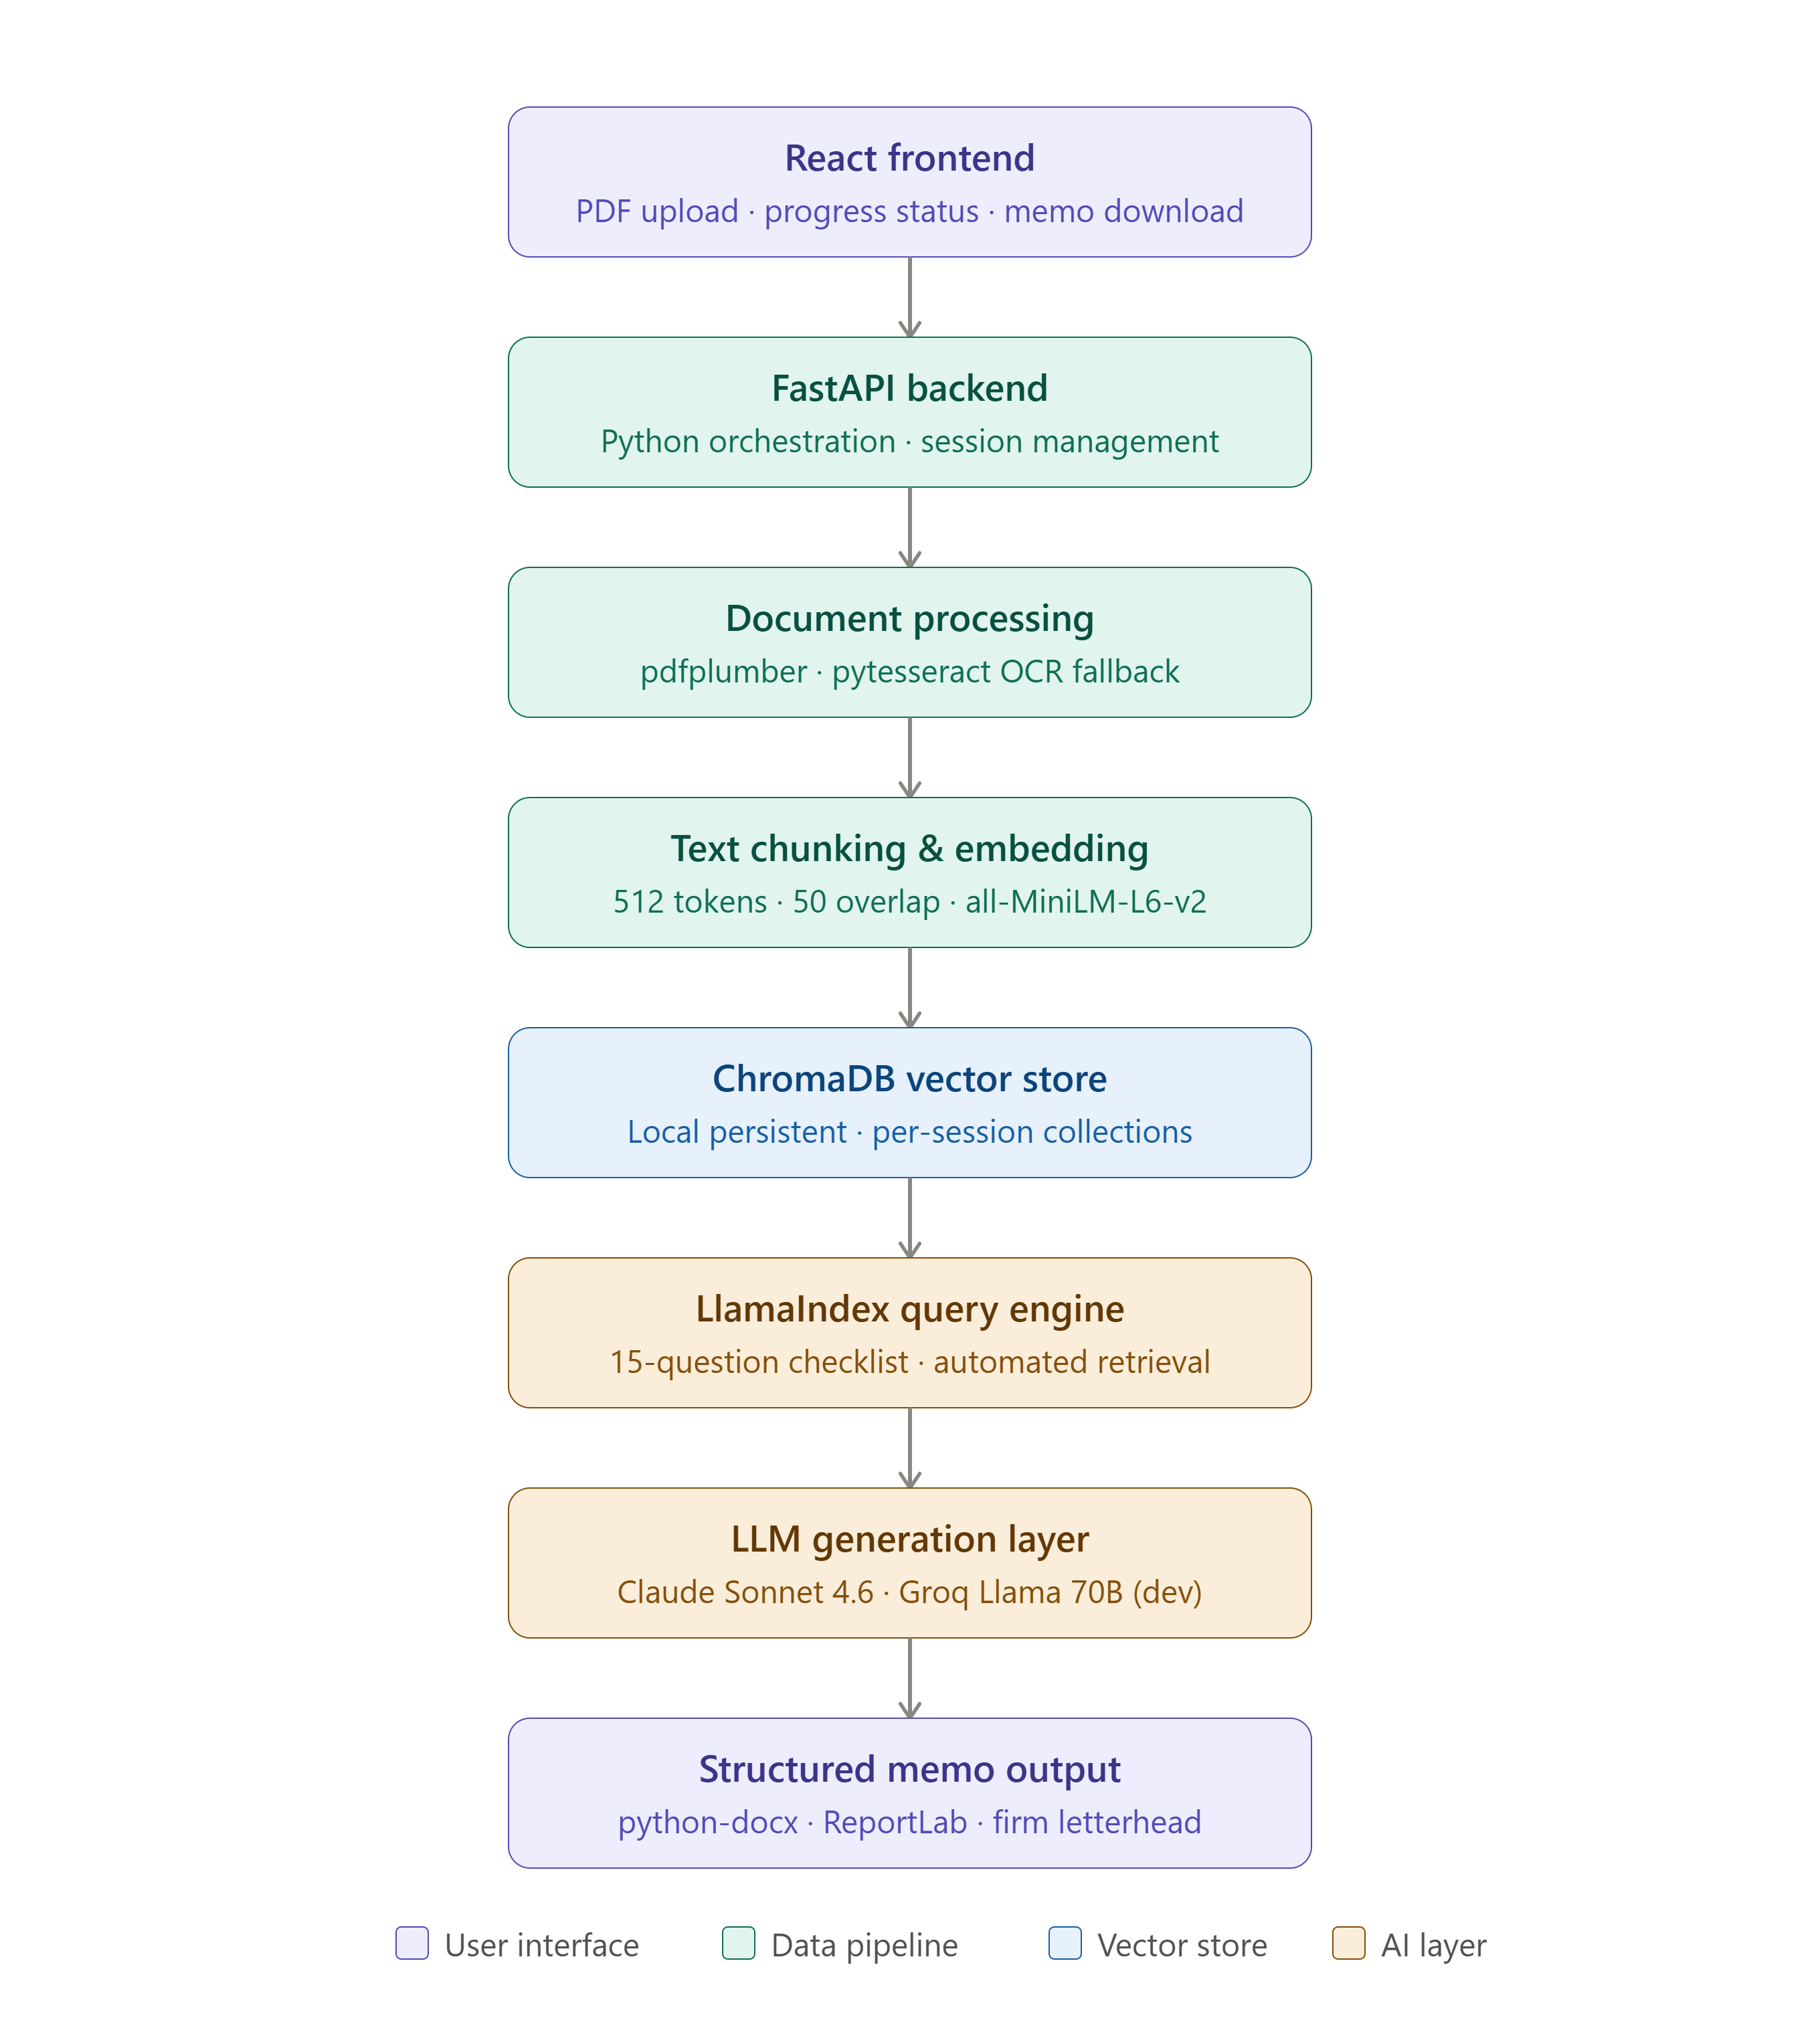
\includegraphics[width=0.62\textwidth]{rag_legal_architecture_flow.png}
    \caption{RAG Legal Document Review System --- Complete Data Flow}
    \label{fig:architecture}
\end{figure}

\subsection{Technology Stack \& Selection Rationale}

\subsubsection{LlamaIndex (over LangChain)}

LlamaIndex is selected as the orchestration framework over LangChain for the
following reasons:

\begin{itemize}[leftmargin=1.5cm]
    \item \textbf{Purpose-built for document retrieval:} LlamaIndex achieved a
    35\% boost in retrieval accuracy in 2025 specifically for document-heavy
    applications---exactly this use case. LangChain is optimised for multi-step
    agentic workflows with tools and memory, which this pipeline does not require.
    \item \textbf{Lower development overhead:} Built-in query engines, routers,
    and fusers designed for RAG mean significantly less boilerplate than an
    equivalent LangChain build.
    \item \textbf{Gentler learning curve:} Its high-level API and focus on data
    connection and querying makes it faster to reach a working pipeline state---
    critical on a 5-day sprint.
    \item \textbf{Native PDF loaders via LlamaHub:} Pre-built data connectors for
    PDFs, databases, and APIs reduce integration work on Day 2.
    \item \textbf{Retrieval performance:} Benchmarks report 2--5$\times$ faster
    lookup times versus generic search pipelines, and 92\% accuracy in retrieval
    benchmarks for document-heavy workflows.
\end{itemize}

\subsubsection{Claude Sonnet 4.6 (Production LLM)}

\begin{itemize}[leftmargin=1.5cm]
    \item \textbf{Pricing:} \$3.00 input / \$15.00 output per million tokens,
    translating to approximately PKR 45 per complete document review.
    \item \textbf{Context window:} 1 million tokens at standard pricing with no
    long-context surcharge---an entire document bundle fits within one context.
    \item \textbf{Structured output compliance:} Claude's instruction-following
    is industry-leading for JSON-format generation, which the memo pipeline
    depends on entirely.
    \item \textbf{Legal document comprehension:} Consistently outperforms peers
    on long-document analysis, clause identification, and contradiction detection.
\end{itemize}

\subsubsection{Groq GPT-OSS 120B (Development \& Testing)}

\begin{itemize}[leftmargin=1.5cm]
    \item \textbf{Migration context:} Groq deprecated \texttt{llama-3.3-70b-versatile}
    on June 30, 2026 (decommission date: August 16, 2026). The project initially
    migrated to \texttt{qwen/qwen3.6-27b} but discovered it is a reasoning model
    that leaks \texttt{<think>} tokens into responses, breaking JSON parsing.
    The project then migrated to \texttt{openai/gpt-oss-120b} --- a non-thinking
    MoE model with 200K TPD free-tier quota --- which produces clean structured
    output required by the legal memo pipeline.
    \item \textbf{Cost:} Completely free on the developer tier---no credit card
    required, no per-token charge.
    \item \textbf{Why GPT-OSS 120B:} Selected as the production replacement
    after Qwen3.6 27B was found to be a reasoning model that leaks internal
    chain-of-thought tokens (\texttt{<think>} blocks) into API responses,
    breaking the structured JSON memo pipeline. GPT-OSS 120B is a non-thinking
    MoE model with clean structured output, 200K tokens per day free-tier quota
    (double the previous model), and benchmark performance matching or surpassing
    proprietary models on reasoning and instruction-following tasks.
    \item \textbf{Speed:} Groq LPU hardware delivers fast inference, making
    demo runs impressively responsive for client presentations.
    \item \textbf{API compatibility:} OpenAI-compatible endpoint---switching to
    Claude Sonnet 4.6 in production requires changing only the base URL and
    API key. Zero other code changes.
\end{itemize}

\subsubsection{HuggingFace paraphrase-multilingual-MiniLM-L12-v2 (Embeddings)}

Free, open-source, runs entirely locally. 384-dimensional dense vectors trained
on 50+ languages including Urdu, with no API dependency, no rate limits, and no
data leaving the machine. Selected over the English-only
\texttt{all-MiniLM-L6-v2} specifically to handle mixed Urdu-English Pakistani
legal documents --- Urdu property descriptions, Khasra references, and
vernacular clauses are embedded and retrieved with full semantic accuracy.

\subsubsection{ChromaDB (Vector Store)}

Zero-infrastructure local vector store. Installed with a single pip command and
operational in three lines of Python. Native LlamaIndex \texttt{ChromaVectorStore}
integration. Persistent local client handles session isolation via UUID-named
collections. The production upgrade path is Qdrant, which provides a near-identical
LlamaIndex API with managed cloud support and horizontal scaling.

\subsubsection{FastAPI (Backend)}

Async-native Python framework. Concurrent uploads handled without blocking.
Auto-generated OpenAPI documentation at \texttt{/docs} for rapid endpoint testing
throughout the sprint. Pydantic request validation built in with no extra
configuration.

% ══════════════════════════════════════════════════════════════════════
\section{Due Diligence Checklist --- Property Transaction}

The following 15-question checklist is the automated review specification for
property transaction due diligence. It is hardcoded as the initial checklist in
the Day 2 build and will be extended to cover loan and acquisition transaction
types on Day 3.

\subsection{Property Transaction Checklist}

\begin{enumerate}[leftmargin=1.5cm, label=\textbf{Q\arabic*.}]
    \item Is the title deed present and registered in the name of the vendor?
    \item Is the property free from all encumbrances, mortgages, charges, or liens?
    \item Are all required NOCs present---LDA/CDA/TMA and all relevant local
    authority approvals?
    \item Are the property boundaries and area measurements consistent across all
    submitted documents?
    \item Is there any ongoing or threatened litigation, court order, or injunction
    against the property?
    \item Is the sale consideration consistent across all documents and supported
    by bank evidence or payment receipts?
    \item Are all signatures, attestations, and notarial certifications present
    and valid?
    \item Is the land use classification consistent with the intended purpose of
    acquisition?
    \item Are utility connections (electricity, gas, water, PTCL) documented and
    registered in the vendor's name?
    \item Are all outstanding property taxes, withholding taxes, and CVT arrears
    disclosed and settled?
    \item Is the vendor's CNIC verified and consistent across all transaction
    documents?
    \item Are there any co-owners, inherited co-sharers, or third-party interests
    in the property?
    \item Is the possession transfer date and handover mechanism explicitly
    documented?
    \item Are all conditions precedent to the transfer clearly identified and
    satisfied?
    \item Is there a registered mutation (Intiqal) on record, or is the transfer
    mode otherwise identified and legally valid?
\end{enumerate}

\subsection{Red Flag Detection Patterns}

Any finding with \texttt{risk\_level: HIGH} is automatically surfaced in the
dedicated Red Flags section of the generated memo.

\begin{table}[H]
\centering
\caption{Red Flag Detection Rules --- Initial Set}
\renewcommand{\arraystretch}{1.3}
\begin{tabularx}{\textwidth}{lXl}
\toprule
\textbf{Pattern} & \textbf{Trigger Condition} & \textbf{Risk Level} \\
\midrule
Missing NOC
    & No NOC document present or issuing authority not identified
    & \textcolor{riskred}{\textbf{HIGH}} \\
Price discrepancy
    & Sale price differs across any two documents by more than 5\%
    & \textcolor{riskred}{\textbf{HIGH}} \\
Undisclosed litigation
    & Court order, injunction, or caveat found in any document
    & \textcolor{riskred}{\textbf{HIGH}} \\
Third-party interest
    & Co-owner or heir mentioned without written consent to transfer
    & \textcolor{riskred}{\textbf{HIGH}} \\
CNIC mismatch
    & Vendor CNIC number differs across any two documents
    & \textcolor{riskred}{\textbf{HIGH}} \\
Missing mutation
    & No Intiqal or equivalent transfer record present
    & \textcolor{accent}{\textbf{MEDIUM}} \\
\bottomrule
\end{tabularx}
\label{tab:redflags}
\end{table}

\subsection{LLM Response Schema}

Each checklist question produces one structured JSON object from the LLM. This
schema drives both the tabular findings section and the red flag detection logic
in the output memo.

\begin{lstlisting}[language=Python, caption={Per-Question LLM Response Format}]
{
  "question_id": 1,
  "question": "Is the title deed present and registered in the vendor's name?",
  "finding": "Title deed (Registry No. 4521/2023) is present and registered in the name of Muhammad Asif Khan, matching vendor CNIC.",
  "reasoning": "Document 1 page 3 contains a registered sale deed bearing Registry No. 4521/2023. The vendor name matches the CNIC provided on page 1. Under Section 17 of the Registration Act 1908, immovable property transactions above PKR 100 must be registered. This requirement is constitutionally grounded in Article 23, which guarantees the right to acquire and dispose of property subject to law.",
  "document_citation": "Uploaded document 1, Page 3, Section A",
  "statutory_citation": "Registration Act 1908, Section 17(1)(b)",
  "constitutional_basis": "Article 23 - Right to acquire and dispose of property",
  "page_number": 3,
  "risk_level": "LOW",       # LOW | MEDIUM | HIGH
  "recommendation": "No action required. Verify stamp duty payment receipt.",
  "missing_documents": [],
  "query_source": "checklist"  # checklist | freeform
}
\end{lstlisting}

% ══════════════════════════════════════════════════════════════════════
\section{Cost Analysis}

\subsection{Per-Review API Cost Model}

A standard property due diligence review involves a 50-page document bundle.
The breakdown below uses Claude Sonnet 4.6 as the production LLM at current
June 2026 pricing.

\begin{table}[H]
\centering
\caption{Per-Review API Cost Breakdown --- Claude Sonnet 4.6}
\renewcommand{\arraystretch}{1.3}
\begin{tabularx}{\textwidth}{Xrrr}
\toprule
\textbf{Component} & \textbf{Tokens} & \textbf{Rate (USD/MTok)} & \textbf{Cost (USD)} \\
\midrule
Document bundle (50 pages $\times$ 500 tok)   & 25,000 & \$3.00  & \$0.075 \\
15 checklist queries ($\times$ avg 500 tok)   &  7,500 & \$3.00  & \$0.023 \\
System prompt overhead                         &  1,000 & \$3.00  & \$0.003 \\
LLM output (15 findings + memo draft)         &  4,000 & \$15.00 & \$0.060 \\
\midrule
\textbf{Total per review}                     & \textbf{37,500} & --- & \textbf{\$0.161} \\
\textbf{Total per review (PKR)}               &        &     & \textbf{$\approx$ PKR~45} \\
\midrule
Embeddings (HuggingFace, runs locally)        & ---    & FREE    & \$0.000 \\
Vector store (ChromaDB, runs locally)         & ---    & FREE    & \$0.000 \\
\bottomrule
\end{tabularx}
\label{tab:apicost}
\end{table}

\begin{calloutbox}{Development Cost During This Sprint}
All sprint development and testing uses Groq GPT-OSS 120B on the free tier
(migrated from Llama 3.3 70B following Groq's June 30, 2026 deprecation notice;
Qwen3.6 27B was trialled but rejected due to reasoning token leakage breaking
JSON parsing). \textbf{Total API development cost: PKR 0.} Free-tier quota:
30 RPM, 1K RPD, 8K TPM, 200K TPD --- sufficient for all testing and demo
workflows.
\end{calloutbox}

\subsection{Monthly SaaS Cost Projections}

\begin{table}[H]
\centering
\caption{Monthly Operational Cost vs Revenue (Production)}
\renewcommand{\arraystretch}{1.3}
\begin{tabularx}{\textwidth}{Xrrr}
\toprule
\textbf{Item}
    & \textbf{Starter}
    & \textbf{Professional}
    & \textbf{Enterprise} \\
\midrule
API cost @ PKR 45/review
    & PKR 1,125 (25 rev.)
    & PKR 4,500 (100 rev.)
    & PKR 9,000 (est.) \\
Hosting (Railway paid tier)
    & PKR 1,400
    & PKR 1,400
    & PKR 2,800 \\
\textbf{Total COGS}
    & \textbf{PKR 2,525}
    & \textbf{PKR 5,900}
    & \textbf{PKR 11,800} \\
\midrule
\textbf{Revenue}
    & \textbf{PKR 15,000}
    & \textbf{PKR 35,000}
    & \textbf{PKR 70,000} \\
\textbf{Gross Margin}
    & \textbf{83\%}
    & \textbf{83\%}
    & \textbf{83\%} \\
\bottomrule
\end{tabularx}
\label{tab:projections}
\end{table}

\subsection{Pricing Model}

\begin{table}[H]
\centering
\caption{SaaS Pricing Tiers for Pakistani Law Firms}
\renewcommand{\arraystretch}{1.3}
\begin{tabularx}{\textwidth}{lXXX}
\toprule
\textbf{Feature}
    & \textbf{Starter --- PKR 15,000/mo}
    & \textbf{Professional --- PKR 35,000/mo}
    & \textbf{Enterprise --- PKR 70,000/mo} \\
\midrule
Monthly reviews     & 25          & 100              & Unlimited \\
Transaction types   & Property    & All 3 types      & All 3 types \\
Custom checklist    & $\times$    & $\checkmark$     & $\checkmark$ \\
Custom letterhead   & $\times$    & $\times$         & $\checkmark$ \\
API access          & $\times$    & $\times$         & $\checkmark$ \\
SLA guarantee       & $\times$    & $\times$         & $\checkmark$ \\
\bottomrule
\end{tabularx}
\label{tab:pricing}
\end{table}

\subsubsection{Client ROI at Professional Tier}

At PKR 35,000 per month, a firm processing 50 reviews per month replaces
approximately PKR 500,000 per month in senior associate time. This delivers a
\textbf{14$\times$ return in month one.} Even at 10 reviews per month, the
subscription pays for itself within the first week of use via time savings alone.

% ══════════════════════════════════════════════════════════════════════
\section{Target Client Identification}

\subsection{Primary Targets for Day 4 Demo}

\subsubsection{Target 1 — Josh and Mak International (Islamabad)}

\begin{itemize}[leftmargin=1.5cm]
    \item \textbf{Location:} No. 01, LG Floor, Josh and Mak International, Park Avenue, Hamza Rd, F-11/1, Islamabad
    \item \textbf{Practice areas:} Legal due diligence, corporate law,
    real estate, M\&A, energy, banking and finance, property transactions
    \item \textbf{Rankings:} Listed on Legal 500 as one of the leading
    law firms in Pakistan
    \item \textbf{Why a fit:} Explicitly provides property due diligence,
    land record searches, and M\&A due diligence as named practice areas.
    The firm has a dedicated due diligence service page on its website.
    \item \textbf{Contact:} aemen@joshandmak.com · www.joshandmakinternational.com
    · +92-304-8734889
    \item \textbf{Transaction type for demo:} Property due diligence
\end{itemize}

\subsubsection{Target 2 — Mumtaz \& Brohi (Islamabad)}

\begin{itemize}[leftmargin=1.5cm]
    \item \textbf{Founded:} 2010
    \item \textbf{Location:} House No. 134, Street No. 60,
    Sector I-8/3, Islamabad
    \item \textbf{Practice areas:} Corporate, commercial, real estate,
    banking, finance, arbitration, intellectual property,
    telecommunications
    \item \textbf{Rankings:} Listed on Legal 500 as one of the top
    law firms of Pakistan; dynamic team of foreign-qualified lawyers
    \item \textbf{Why a fit:} Full transactional practice covering all
    three target transaction types (property, loan, acquisition).
    Serves multinational corporations, financial institutions, and
    commercial enterprises --- the exact client profile that demands
    fast due diligence turnaround.
    \item \textbf{Contact:} info@mumtazandbrohi.com · www.mumtazandbrohi.com
    · +92-51-4800851
    \item \textbf{Transaction types for demo:} Property due diligence
    (primary), acquisition due diligence (secondary)
\end{itemize}

\subsection{Approved Outreach Script}

\begin{scriptbox}
``Salam, I am an AI engineering intern working on a legal technology project.
We have built a system that automates first-pass property due diligence
review---it takes 50 pages of legal documents and produces a structured review
memorandum in under 5 minutes. We are looking for a law firm to conduct a live
demonstration with this week. Would you have 30 minutes for a quick
demonstration? There is no cost and no commitment involved.''
\end{scriptbox}

\subsection{Client Feedback Form (Post-Demo)}

\begin{table}[H]
\centering
\caption{Day 4 Client Feedback Form Template}
\renewcommand{\arraystretch}{1.5}
\begin{tabularx}{\textwidth}{lX}
\toprule
\textbf{Field} & \textbf{Response} \\
\midrule
Firm name                           & \\
Contact person \& designation       & \\
Demo date \& format                 & \\
Transaction type demonstrated       & \\
What they liked                     & \\
Requested changes                   & \\
Interest level (1--5)               & \\
Follow-up scheduled?                & \\
\bottomrule
\end{tabularx}
\end{table}

% ══════════════════════════════════════════════════════════════════════

\vspace{1.5cm}
\vfill

\begin{center}
    {\color{primary}\rule{0.55\textwidth}{0.5pt}}\\[0.35cm]
    {\small\color{darkgray}
    Legal RAG System \textperiodcentered{}
    Day 1 Submission \textperiodcentered{}
    Pair B \textperiodcentered{}
    AI/ML Internship Program}\\[0.15cm]
    {\small\color{darkgray} Confidential \textperiodcentered{} Internal Document}
\end{center}

\end{document}